\chapter{Frontend Implementation and Design}
\label{chap:ch6}

\par The QuickShift frontend was built as an application using React 18 and TypeScript, with Vanilla CSS for styling. The guiding design principles were operational clarity and low friction: the interface should allow a non-technical store manager to generate schedules,  review absences, and manage staff without requiring training or documentation. At the same time, the interface must expose the full complexity of the underlying workflows — replacement chains, leave approval with balance tracking, manual shift corrections — through well-structured, action-oriented components.

%-----------------------------------------------------------
\section{Project Structure}
%-----------------------------------------------------------
\par React was chosen for its component model, which maps naturally onto the page-and-panel structure of the application. TypeScript adds static typing that catches API contract mismatches at development time, which is particularly valuable when the backend response shapes evolve as new features are added. Vite is used as the build tool, providing fast hot-module replacement during development and a compact production bundle.

\par API communication is handled through the Axios library \cite{axios}, with a centralized instance configured with the base URL from an environment variable. All authenticated requests attach the JWT stored in \texttt{localStorage} via a request interceptor, so individual service functions do not need to manage the Authorization header explicitly.  Unauthorized (401) responses are handled in the authentication layer when fetching the current user and triggering the logout flow to prevent stale credentials from persisting in the UI.

\par Authentication state is managed through a custom \texttt{useAuth} hook backed by React context. The hook exposes the current user, authentication flags, and helpers to store or clear the JWT. Login flows call the API and then store the received token via the context helper, while logout clears storage and auth state; routing logic then redirects unauthenticated users to the public pages. Components consume the hook to conditionally render content based on the user’s role and authentication status.

%-----------------------------------------------------------
\subsection{Routing and Route Protection}
%-----------------------------------------------------------
\par Client-side routing is handled by React Router v6. The route configuration is centralized in the main application component, with a \texttt{ProtectedRoute} wrapper component that checks the current authentication state before rendering the target page. Unauthenticated users attempting to access protected routes are redirected to the login page; authenticated users attempting to access the login or registration pages are redirected to the schedule page.

\par Role-based routing is layered on top of authentication protection. Certain pages such as the store management screen are accessible only to administrators; the schedule and notifications pages are accessible to both managers and employees, but render different content and controls depending on the role. This approach keeps the routing table simple while still enforcing role-appropriate access at the page level.

%-----------------------------------------------------------
\section{Calendar-Centric Scheduling Interface}
%-----------------------------------------------------------
\par The calendar page is the operational hub of the application. It renders a monthly grid in which each cell corresponds to one day, and each cell may contain one or more shift cards representing scheduled employees. Shift cards display the employee's full name, the shift type, and a color-coded status indicator that distinguishes between \texttt{SCHEDULED}, \texttt{ABSENT}, and \texttt{REPLACEMENT} shifts at a glance.

\par The calendar supports two navigation dimensions: the user can move forward or backward by month using arrow controls, and can also switch between stores if they have administrator privileges. The underlying API calls are parameterized by year, month, and optionally store ID, so the calendar always shows exactly the data relevant to the selected view.

\par Schedule generation is triggered from a button in the calendar header.Upon submission by the manager of the respective store, the frontend calls the generation endpoint and re-fetches the shift list on success, so the calendar updates immediately without a full page reload.

\begin{figure}[H]
    \centering
    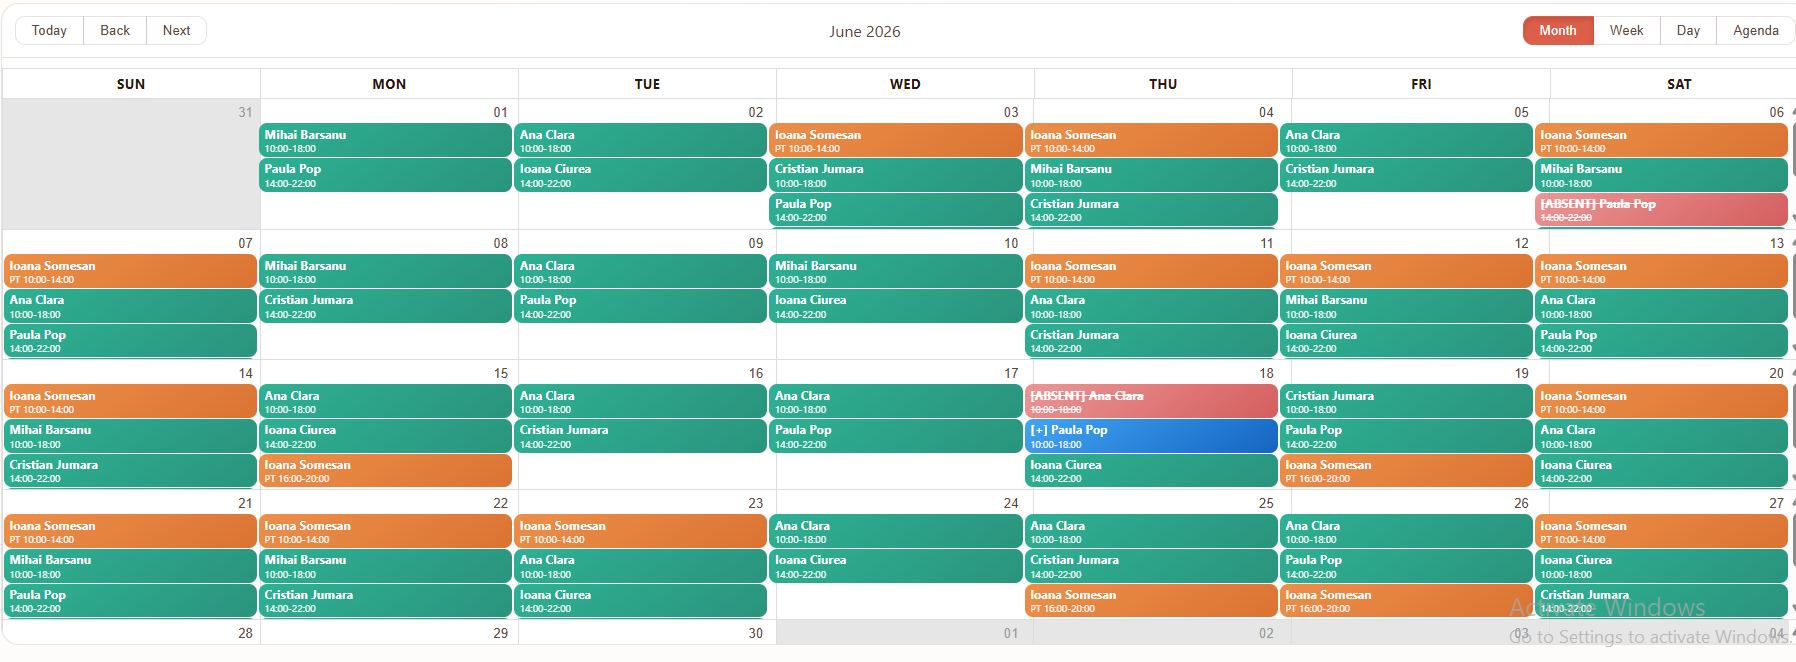
\includegraphics[width=1\linewidth]{Schedule.png}
    \caption{Main Schedule viewpoint}
    \label{fig:placeholder}
\end{figure}

\subsubsection*{Manual shift addition}

\par Managers can add individual shifts by clicking on the \texttt{Manage Shifts} button and selecting a date for the shift. The form first fetches the list of eligible employees for the selected date and shift type from the backend, populating the employee selector with only valid choices. This server-driven eligibility check ensures that the constraint logic described in Chapter 4 is enforced at the point of selection rather than only at submission time, which reduces the likelihood of a rejected submission and provides clearer guidance to the manager.

\par After selecting an employee and confirming, the frontend calls the shift creation endpoint and re-renders the relevant calendar cell on success. An error returned by the backend (for example, if the employee becomes ineligible between the time the form was opened and the time of submission) is displayed inline in the form panel.

\subsubsection*{Shift deletion}

\par Managers can delete a shift by clicking on the remove action from the same \texttt{Manage Shifts} menu. There, all the scheduled shifts for the selected date, alongside the addition option, can be viewed. The delete endpoint is called and the card is removed from the calendar grid on success. A confirmation step is deliberately omitted to keep the interaction smooth (if the manager manually updated that shift, it is necessary to respect it); instead, the employee receives an automatic \texttt{[SHIFT REMOVED]} notification via the system, which serves as a record of the change.

\begin{figure}[H]
    \centering
    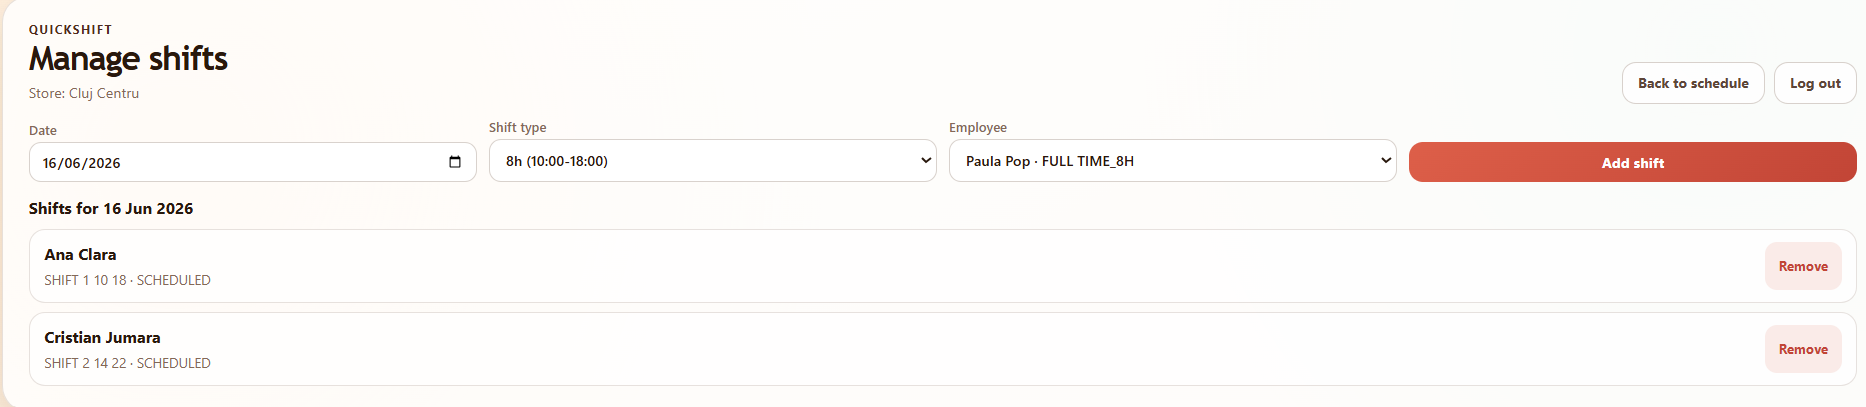
\includegraphics[width=0.5\linewidth]{Manual Shift.png}
    \caption{Manual Shift manipulations for managers overview}
    \label{fig:placeholder}
\end{figure}

%-----------------------------------------------------------
\section{My Shifts Page and Employee Self-Service}
%-----------------------------------------------------------
\par Employees interact with the system primarily through the \emph{Manage my shifts} page, which presents their personal shift schedule in a combined calendar and list view. The page shows all shifts assigned to the logged-in employee across the current and upcoming months, with the same status color coding used in the manager calendar.

\par From this page, employees can report absence for any future shift in a \texttt{SCHEDULED} or \texttt{REPLACEMENT} status. The report form asks for an optional reason, which is stored on the absence request and visible to the manager. Submitting the report creates the absence request in the backend and sends the manager notification described in Chapter 4; the shift's status does not change immediately, since the system waits for manager acknowledgment before marking it as \texttt{ABSENT}.

\par Employees can also submit leave requests from this page. A date range picker scoped to the next calendar month allows them to select the desired period, and the form displays their current remaining leave balance alongside the estimated deductible days for the selected range (calculated from the 5/7 calendar-to-working-day ratio). This real-time estimate helps employees make informed decisions before submitting, reducing the frequency of requests that exceed the available balance.

\begin{figure}[H]
    \centering
    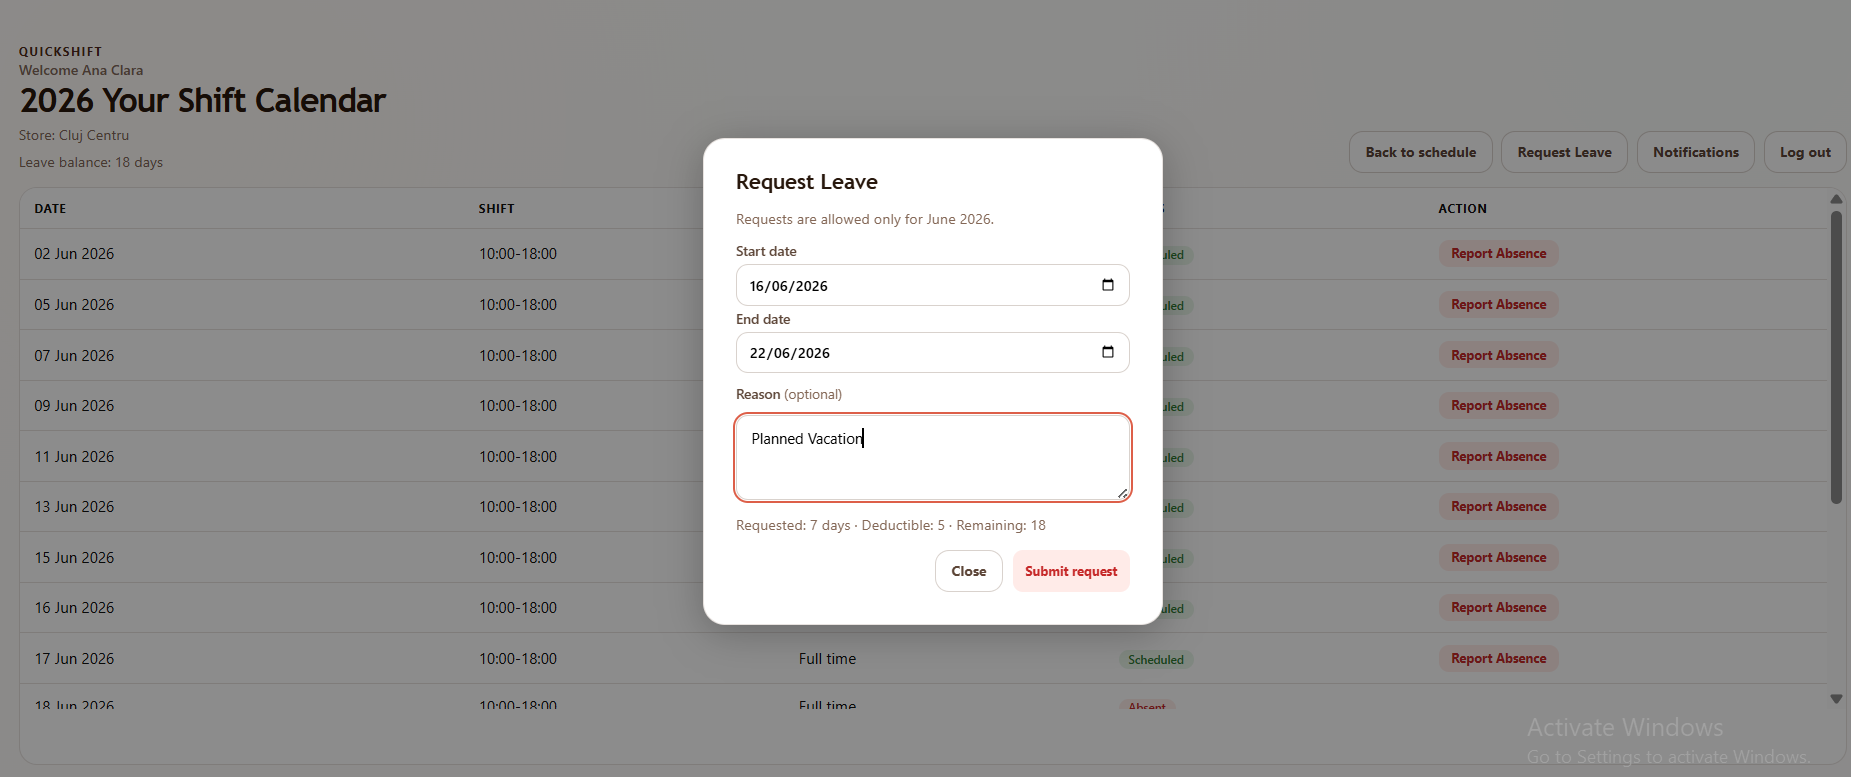
\includegraphics[width=1\linewidth]{LeaveRequest.png}
    \caption{Leave request option on the manage shifts page}
    \label{fig:placeholder}
\end{figure}

%-----------------------------------------------------------
\section{Notifications Page and Workflow Actions}
%-----------------------------------------------------------
\par The notifications page is the primary coordination surface between managers and employees. It renders a chronological list of all unread notifications for the current user on the main dashboard, with read notifications visible but visually de-emphasized on the designated notifications page. Each notification card displays the message text, the store name, and the creation timestamp.

\par The key design challenge of the notifications page is that different notification types require fundamentally different action controls, and the state of those controls must be maintained as the user interacts with them without causing the entire list to re-fetch on every action. This is solved by maintaining per-notification action state in three separate state maps within the page component: one for acknowledgment actions (absence requests), one for leave decisions, and one for replacement offer actions. Each map is keyed by notification ID, so updates to one notification do not disturb the display state of others.

\subsubsection*{Absence acknowledgment}

\par Notifications prefixed with \texttt{[ABSENCE REQUEST]} render an \emph{Acknowledge \& Replace} button. Clicking it calls the acknowledgment endpoint and updates the notification's local state to show a result message: either a success message naming the replacement employee, or a warning if no replacement was found. In the success case, the shift proposal is sent through a notification to that employee, and if they accept, a follow-up notification is sent to the manager with the person that accepted the shift.

\subsubsection*{Leave request decisions}

\par Notifications prefixed with \texttt{[LEAVE REQUEST]} render two buttons: \emph{Approve leave} and \emph{Deny}. The deny flow opens an inline panel in which the manager can enter an optional reason before confirming. In the approved state, the notification transitions to a success message and the employee also receives a confirmation of the leave request being approved. The amount of leave days remaining in the employee's balance is deducted immediately, and upon generation of the month in which the leave was requested, the employee will not be considered for any shifts in the requested period.

\subsubsection*{Replacement offer acceptance and denial}

\par Notifications prefixed with \texttt{[REPLACEMENT OFFER]} are received by employees and render \emph{Approve extra shift} and \emph{Deny} buttons. Clicking either button calls the corresponding endpoint and marks the notification as read. The system then handles the downstream consequences (creating the replacement shift on acceptance, or triggering the next automated search on denial) server-side, and the manager receives a follow-up notification reflecting the outcome.

\subsubsection*{No replacement alerts}

\par Notifications prefixed with \texttt{[NO REPLACEMENT]} are received by managers when no eligible replacement could be found for an absent shift. These notifications render a \emph{Find another replacement} button, which triggers a new automated search from the current state of the employee pool (potentially with different constraint states compared to when the original search ran). They also render a \emph{Mark as read} button so that managers can dismiss the alert after arranging a manual resolution outside the system. This dismissal path is essential for the system to remain usable when all automated options have been exhausted.

%-----------------------------------------------------------
\section{Authentication Pages and Account Recovery}
%-----------------------------------------------------------
\par The login page presents a standard email and password form with inline error feedback for authentication failures. Successful login stores the JWT and decoded user payload in \texttt{localStorage} and redirects the user to the schedule page.

\par The registration page is available to employees who self-onboard. It collects full name, email, password, contract type, shift preference, and optionally a store selection. A password confirmation field with client-side match validation reduces the likelihood of registration failures caused by typing errors. On successful registration, the user is automatically logged in and redirected to their personal shift page.

\par The forgot-password page accepts an email address and triggers the backend reset flow. The form does not indicate whether the supplied email corresponds to an existing account, preventing account enumeration attacks. After submission, the user is shown a generic confirmation message instructing them to check their email. The reset page, linked from the email, accepts the new password and its confirmation, validates both client-side for match and minimum length, and submits to the backend token validation and update endpoint.

\par The change-password page for authenticated users requires the current password, the new password, and a confirmation. Since users are already authenticated for this functionality, it does not require any restrictive attention, like the forgot password does.

%-----------------------------------------------------------
\section{Role-Specific Navigation and UI Adaptation}
%-----------------------------------------------------------
\par Navigation is rendered conditionally based on the current user's role. The navigation bar items, action buttons, and page sections visible to each role are as follows:

\begin{itemize}
    \item \textbf{Employees} see their personal shift calendar, the leave request form, the absence reporting controls, and the notifications page for replacement offer decisions.
    \item \textbf{Managers} see the store schedule calendar with generation, manual add, and delete controls; the notifications page with absence acknowledgment and leave decision controls; and the employee list for their store.
    \item \textbf{Administrators} see all of the above(except manual shift manipulation) plus the store management page, the manager provisioning form, and a global employee view across any chosen store.
\end{itemize}

\par Role-specific UI is handled within the components themselves: they read the user role from \texttt{useAuth} and conditionally render controls (e.g., manager-only actions) as needed, while routing primarily gates access based on authentication status rather than role-based route splits.\cite{fireactUseAuth}

%-----------------------------------------------------------
\subsection{Store Management and Administrator Interface}
%-----------------------------------------------------------
\par The store management page is accessible only to administrators. It provides a tabbed interface covering three areas: store creation, employee listing with store assignment, and manager provisioning.

\par Store creation requires a store name, a location identifier and a busy day threshold - which can then be updated by the managers depending on the stores' sales. After creation, the store appears immediately in the store selector used throughout the application. The administrator can then assign a manager to the store through the provisioning form, which requires an email address and the target store. The provisioning action creates the manager account, sends the onboarding email, and links the account to the selected store in a single operation.

\par The employee listing shows all registered employees grouped by store, with their contract type, shift preference, and current leave day balance visible.

\begin{figure}[H]
    \centering
    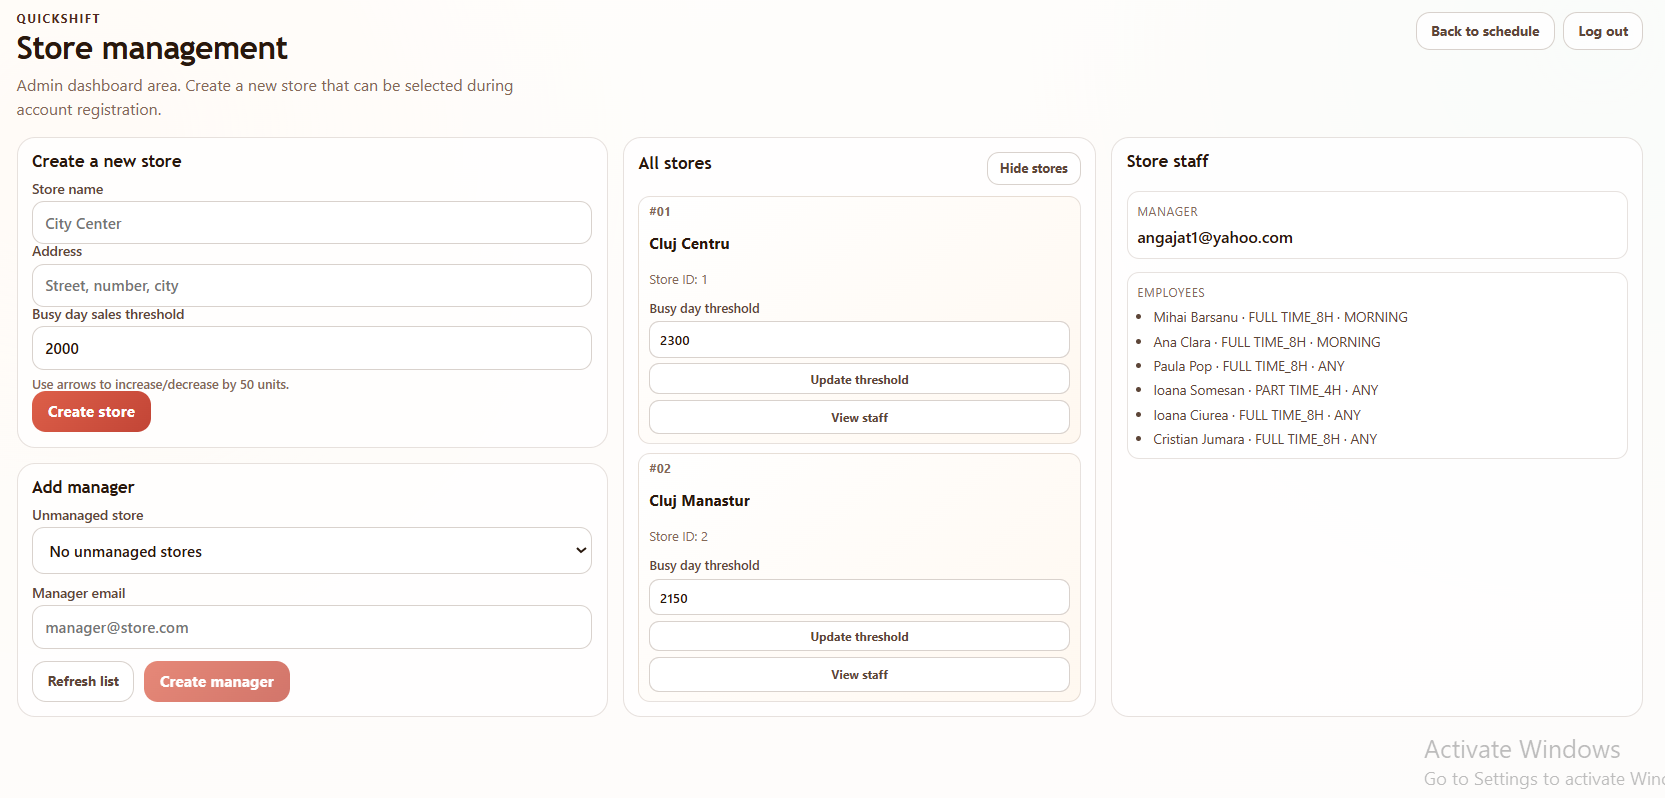
\includegraphics[width=0.7\linewidth]{ManageStores.png}
    \caption{Manage stores page overview}
    \label{fig:placeholder}
\end{figure}

%-----------------------------------------------------------
\section{Client-Side State Management Strategy}
%-----------------------------------------------------------
\par The application does not use a global state management library such as Redux. Instead, state is organized at the page level using React's built-in \texttt{useState} and \texttt{useEffect} hooks. Authentication state is the only globally shared state, distributed through a context provider.\cite{reactUseEffect}, \cite{reactUseState}

\par This choice reflects the scale of the application: the data flows are straightforward, and each page typically fetches the data it needs directly. The overhead of a global store would exceed the complexity it resolves. The trade‑off is that some data is re‑fetched more often than strictly necessary (for example, the notification list after each action), but this keeps the UI consistent with the server state and is acceptable for the expected usage volume.
\par Local action state (pending flags, error messages, inline results) is tracked in per-notification state maps as described in the notifications section, allowing fine-grained loading and error feedback without blinking the entire list on each interaction.

%-----------------------------------------------------------
\section{Styling Philosophy and Visual Design}
%-----------------------------------------------------------
\par The styling is implemented entirely in Vanilla CSS \cite{cssVanillaLayout} using custom properties (CSS variables) for the color palette and spacing scale. This allows the visual design to be adjusted globally by modifying a small set of root variables, without hunting for hardcoded values scattered across stylesheets.

\par The color system distinguishes between states through consistent cues: green for success and approved statuses, amber for warnings and pending states, red for errors and absent statuses, and a neutral dark palette for the base layout. Status badges on shift cards use these colors directly, so a manager scanning the calendar can identify problematic days at a glance without reading the text of each card.

\par Typography uses the Inter font family loaded from Google Fonts. Inter was chosen for its high legibility at small sizes and its wide character coverage, which is important for displaying names and dates in compact calendar cells. Body text is set at a size and line-height optimized for reading-dense content such as notification messages.

\par Micro-interactions are implemented with CSS transitions on buttons, cards, and panel slide-ins. These transitions are short (100–200 ms) and target only opacity and transform properties, which are GPU-composited and do not cause layout recalculation. The result is a perceived responsiveness that makes the interface feel immediate even when network latency introduces a short delay between action and data update.

%-----------------------------------------------------------
\section{Error Handling and User Feedback Patterns}
%-----------------------------------------------------------
\par Every API call in the application is wrapped in a try/catch block with explicit handling for the most likely error cases. Axios errors with a string \texttt{response.data} field are displayed directly as the error message, since the backend uses this format for business logic errors (validation failures, constraint violations). Generic network or server errors fall back to a predefined message that is informative but does not expose internal details.

\par Loading states are communicated through button label changes (\emph{Processing...}, \emph{Loading...}) rather than spinner overlays. This approach keeps the interface visually stable during pending operations and avoids the jarring experience of layout shifts caused by adding or removing overlay components. Buttons are disabled during pending states to prevent duplicate submissions.

\par Success states are communicated inline within the component that performed the action, typically replacing the action button with a confirmation message. This keeps the feedback spatially close to the control the user interacted with, which is consistent with the principle of minimal cognitive distance between action and response.

